\section{Evaluation}
\label{eval}
%Evaluation section...
%
%Length: 3-4 pages (graphs take a lot of space!)
%
%Tell reader what to expect.
%
%Eval is "proof" that your design is good.
%MATCH eval goals with design goals.
%
%Eval section is easier to write, but longest one to produce
%results for.  Whereas design section has complex structure, eval
%is more 'flat'.
%
%Structure:
%
%1.  list eval goals, should match design goals
%
%2.  briefly list how you plan to prove those goals.
%
%3.  describe your testbed: h/w + s/w platform to run tests on.
%Give enough detail so it can be reproduced by ANYONE.
%
%4.  describe your benchmarks in detail:
%
%(4a) Micro benchmarks: test specific feature (e.g., read or
%write performance).  Usually u-bench are designed to highlight
%worst/best case behavior of your system.  Be to list both best
%and worst.
%
%(4b) Macro benchmarks (general purpose benchmarks): test whole
%system (e.g., run a Web server exerciser, or TPC for database).
%
%Some tests should compare YOUR system to past systems, or a
%"before and after" comparison.
%
%For every possible variable in your system, design a set of
%independent tests (re: compression study's dimensions).  Justify
%need to vary each variable (the more variables, the more
%experiments you have to run).
%
%5.  Describe your benchmarking methodology
%
%Statistical stability: how many times you run each test? do you
%compute standard deviations, half-width intervals (for student-t
%distribution), RMS, or other metric of stability?  Say how many
%times you ran each test, and what were the stability metrics.
%
%Ex."we ran every test at least 10 times, and computed the
%standard deviation as a percentage of the mean.  In all cases,
%the percentage was less than 5\%, unless otherwise noted."
%
%6.  List every benchmark result, for each test
%
%(a) a graph or table or other figure, plus caption.
%(b) followed by an explanation of the figure: say what one sees
%    in the figure, then explain WHY it is so.
%
%7.  Optional: if eval section longer than usual, end it with a
%one-paragraph summary of eval results.

\paragraph{Evaluation Goals}
We aimed to perform a thorough benchmarking of existing BFS algorithms
for energy efficiency and analyse the results in terms of MEM, ENERGY,
POWER and CACHE performance.
\begin{itemize}
\item
\textbf{BFS implementations}\\
We have collected \emph{six} BFS implementations, verified their
corectness.
\item
\textbf{Dataset}\\
We have collected \emph{eleven} graph datasets from \emph{Florida
Sparse Matrix} database.  Pre-processed them for algorithm conformity.
\item
\textbf{Benchmarking}\\
We have benchmarked the algorithms by running them on our collected
graph datasets and measured the readings for our relevant parmeters.
\end{itemize}

\paragraph{Results}
We run the experiments and measure the MEM, ENERGY, POWER, L2CACHE and
L3CACHE miss using \emph{likwid-perfctr} and \emph{likwid-pwermeter}.


%\begin{table}[th]
%\begin{center}
%    \begin{tabular}{| l | l | l | l | l | l | l |}
%    \hline
%	Dataset & Algo1 & Algo2 & Algo3 & Algo4 & Algo5 & Algo6\\ \hline
%	gre\_1107 & 1.19 & 5.17 & 0.93 & 1.35 & 1.25 & 1.33 \\ \hline
%	cell1 & 4.16 & 20.89 & 2.09 & 3.62 & 4.53 & 4.73\\ \hline
%	appu & 172.91 & 112.16 & 92.21 & 8.92 & 171.13 & 175.07\\ \hline
%	conf6 & 185.58 & 119.82 & 103.45 & 9.98 & 191.85 & 185.86\\ \hline
%	dblp & 244.31 & 148.81 & 124.70 & 13.96 & 241.30 & 235.15\\ \hline
%	amazon & 220.47 & 136.91 & 109.67 & 16.16 & 224.48 & 208.35\\ \hline
%	fem & 2091.23 & 1182.47 & 1119.56 & 87.31 & 2092.19 & 2102.01\\ \hline
%	Chevron4 & 645.25 & 481.38 & 338.31 & 76.22 & 642.99 & 640.16\\ \hline
%	cage14 & 2953.03 & 1626.01 & 1555.99 & 129.44 & 2942.22 & 2973.07\\ \hline
%	cage15 & 11267.14 & 6200.88 & 5936.38 & 499.53 & 11390.66 & 11452.49\\ \hline
%	delaunay & 12762.75 & 7124.39 & 6682.38 & 751.73 & 12893.38 & 12677.84\\ \hline
%    \end{tabular}
%\end{center}
%\caption{\capfont ENERGY readings}
%\label{tab:Table1}
%\end{table}
%
%
%
%\begin{table}[th]
%\begin{center}
%    \begin{tabular}{| l | l | l | l | l | l | l |}
%    \hline
%	Dataset & Algo1 & Algo2 & Algo3 & Algo4 & Algo5 & Algo6\\ \hline
%	gre & 63.82 & 67.15 & 60.99 & 82.85 & 63.11 & 66.32 \\ \hline
%	cell1 & 67.53 & 67.51 & 60.55 & 111.95 & 71.61 & 71.36\\ \hline
%	appu & 72.37 & 64.35 & 77.86 & 111.53 & 73.79 & 74.17\\ \hline
%	conf6 & 74.85 & 65.35 & 78.20 & 113.69 & 72.82 & 75.78\\ \hline
%	dblp & 76.69 & 67.59 & 80.60 & 117.85 & 76.26 & 73.07\\ \hline
%	amazon & 70.46 & 65.29 & 77.67 & 126.79 & 76.42 & 76.25\\ \hline
%	fem & 77.09 & 73.49 & 78.85 & 142.76 & 76.03 & 76.07\\ \hline
%	Chevron4 & 77.15 & 68.78 & 78.10 & 160.25 & 78.93 & 77.72\\ \hline
%	cage14 & 77.31 & 73.71 & 78.63 & 156.93 & 77.08 & 77.23\\ \hline
%	cage15 & 77.06 & 74.79 & 77.71 & 176.09 & 77.70 & 77.68\\ \hline
%	delaunay & 76.83 & 74.16 & 78.93 & 181.46 & 77.45 & 76.89\\ \hline
%    \end{tabular}
%\end{center}
%\caption{\capfont POWER readings}
%\label{tab:Table2}
%\end{table}


\begin{table*}[th]
\begin{center}
    \begin{tabular}{| l | l | l | l | l | l | l |}
    \hline
	Dataset & Algo1 & Algo2 & Algo3 & Algo4 & Algo5 & Algo6\\ \hline
	Gre & \cellcolor{blue!25}3.46 & 22.03 & 4.25 & 4.2 & 5.4 & 5.64 \\ \hline
	Cell1 & 10.57 & 99.92 & \cellcolor{blue!25}3.65 & 56.92 & 14.37 & 16.79\\ \hline
	Appu & 150.85 & 152.95 & \cellcolor{blue!25}121.79 & 445.63 & 123.45 & 130.12\\ \hline
	Conf6 & 155.97 & 153.01 & \cellcolor{blue!25}133.67 & 473.59 & 145.70 & 145.20\\ \hline
	Dblp & 333.22 & 282.73 & \cellcolor{blue!25}193.29 & 682.99 & 291.98 & 268.84\\ \hline
	Amazon & 322.82 & 317.66 & \cellcolor{blue!25}173.32 & 699.97 & 246.82 & 255.30\\ \hline
	Fem & 1607.10 & 2264.73 & \cellcolor{blue!25}1398.64 & 6774.77 & 1616.92 & 1573.88\\ \hline
	Chevron & 697.41 & 920.61 & \cellcolor{blue!25}577.01 & 3145.14 & 695.26 & 764.84\\ \hline
	Cage14 & 2830.57 & 3837.75 & \cellcolor{blue!25}2060.95 & 11183.9 & 2876.8 & 2887.03\\ \hline
	Cage15 & 10850.6 & 15121.6 & \cellcolor{blue!25}8351.24 & 44794.6 & 11106.5 & 11088.2\\ \hline
	Delaunay & 14667.8 & 13353.9 & \cellcolor{blue!25}9447.41 & 52910.3 & 13614.7 & 13194.1\\ \hline
    \end{tabular}
\end{center}
\caption{\capfont MEM readings in MB}
\label{tab:Table3}
\end{table*}

\begin{table*}[th]
\begin{center}
    \begin{tabular}{| l | l | l | l | l | l | l |}
    \hline
	Dataset & Algo1 & Algo2 & Algo3 & Algo4 & Algo5 & Algo6\\ \hline
	Gre & \cellcolor{blue!25}0.8 & 13.857 & 2.0 & 0.59 & 2.86 & 1.0\\ \hline
	Cell1 & 3.0 & 57.2 & \cellcolor{blue!25}1.0 & 7.17 & 7.78 & 7.0\\ \hline
	Appu & 2.0 & 5.34 & 6.0 & \cellcolor{blue!25}0.68 & 1.66 & 2.0\\ \hline
	Conf6 & 8.0 & 10.41 & 5.0 & \cellcolor{blue!25}4.44 & 12.3 & 12.0\\ \hline
	Dblp & 7.0 & 25.22 & 8.0 & \cellcolor{blue!25}4.99 & 16.5 & 11.0\\ \hline
	Amazon & 15.0 & 27.04 & 12.0 & \cellcolor{blue!25}11.5 & 34.3 & 21.0\\ \hline
	Fem & \cellcolor{blue!25}12.0 & 39.46 & 41.0 & 29.9 & 18.5 & 29.0\\ \hline
	Chevron & \cellcolor{blue!25}44.0 & 291.27 & 46.0 & 132.0 & 112.56 & 96.0\\ \hline
	Cage14 & 43.0 & 66.06 & \cellcolor{blue!25}41.0 & 54.4 & 57.65 & 49.0\\ \hline
	Cage15 & 154.0 & 177.48 & \cellcolor{blue!25}121.0 & 164.0 & 172.15 & 166.0\\ \hline
	Delaunay & 271.0 & 785.63 & \cellcolor{blue!25}265.0 & 513.0 & 444.17 & 648.0\\ \hline
    \end{tabular}
\end{center}
\caption{\capfont Running time in ms}
\label{tab:Table4}
\end{table*}

\begin{table*}[th]
\small
\centering
%\begin{tabularx}{\linewidth}{|c|c|c|c|c|c|c|X|}

\begin{tabular}{ c|c|c|c|c|c|c|c|c|c|c|c|c| }
\hline
\multicolumn{1}{|c|}{\textbf{Dataset}} &
\multicolumn{6}{c}{\textbf{ENERGY}}&
  \multicolumn{6}{|c|}{\textbf{POWER}} \\
  \cline{2-13}
  \multicolumn{1}{|c|}{} &
  Algo1 & Algo2 & Algo3 & Algo4 & Algo5 & Algo6 & Algo1 & Algo2 & Algo3 & Algo4 & Algo5 & Algo6\\\hline
  \multicolumn{1}{|c|}{\textbf{Gre}}
& 1.19 & 5.17 & \cellcolor{blue!25}0.93 & 1.35 & 1.25 & 1.33 & 63.82 & 67.15 & \cellcolor{green!25}60.99 & 82.85 & 63.11 & 66.32 \\ \hline
  \multicolumn{1}{|c|}{\textbf{Cell1}}
& 4.16 & 20.89 & \cellcolor{blue!25}2.09 & 3.62 & 4.53 & 4.73 & 67.53 & 67.51 & \cellcolor{green!25}60.55 & 111.95 & 71.61 & 71.36\\ \hline
  \multicolumn{1}{|c|}{\textbf{Appu}}
& 172.91 & 112.16 & 92.21 & \cellcolor{blue!25}8.92 & 171.13 & 175.07 & 72.37 & \cellcolor{green!25}64.35 & 77.86 & 111.53 & 73.79 & 74.17\\ \hline
  \multicolumn{1}{|c|}{\textbf{Conf6}}
& 185.58 & 119.82 & 103.45 & \cellcolor{blue!25}9.98 & 191.85 & 185.86 & 74.85 & \cellcolor{green!25}65.35 & 78.20 & 113.69 & 72.82 & 75.78\\ \hline
  \multicolumn{1}{|c|}{\textbf{Dblp}}
& 244.31 & 148.81 & 124.70 & \cellcolor{blue!25}13.96 & 241.30 & 235.15 & 76.69 & \cellcolor{green!25}67.59 & 80.60 & 117.85 & 76.26 & 73.07\\ \hline
  \multicolumn{1}{|c|}{\textbf{Amazon}}
& 220.47 & 136.91 & 109.67 & \cellcolor{blue!25}16.16 & 224.48 & 208.35 & 70.46 & \cellcolor{green!25}65.29 & 77.67 & 126.79 & 76.42 & 76.25\\ \hline
  \multicolumn{1}{|c|}{\textbf{Fem}}
& 2091.23 & 1182.47 & 1119.56 & \cellcolor{blue!25}87.31 & 2092.19 & 2102.01 & 77.09 & \cellcolor{green!25}73.49 & 78.85 & 142.76 & 76.03 & 76.07\\ \hline
  \multicolumn{1}{|c|}{\textbf{Chevron4}}
& 645.25 & 481.38 & 338.31 & \cellcolor{blue!25}76.22 & 642.99 & 640.16 & 77.15 & \cellcolor{green!25}68.78 & 78.10 & 160.25 & 78.93 & 77.72\\ \hline
  \multicolumn{1}{|c|}{\textbf{Cage14}}
& 2953.03 & 1626.01 & 1555.99 & \cellcolor{blue!25}129.44 & 2942.22 & 2973.07 & 77.31 & \cellcolor{green!25}73.71 & 78.63 & 156.93 & 77.08 & 77.23\\ \hline
  \multicolumn{1}{|c|}{\textbf{Cage15}}
& 11267.14 & 6200.88 & 5936.38 & \cellcolor{blue!25}499.53 & 11390.66 & 11452.49 & 77.06 & \cellcolor{green!25}74.79 & 77.71 & 176.09 & 77.70 & 77.68\\ \hline
  \multicolumn{1}{|c|}{\textbf{Delaunay}}
& 12762.75 & 7124.39 & 6682.38 & \cellcolor{blue!25}751.73 & 12893.38 & 12677.84 & 76.83 & \cellcolor{green!25}74.16 & 78.93 & 181.46 & 77.45 & 76.89\\ \hline
\end{tabular}

%\end{tabularx}
\caption{\capfont ENERGY (in Joules) and POWER (in Watts) readings }
\label{tab:Table5}
\end{table*}


\begin{table*}[th]
\small
\centering
%\begin{tabularx}{\linewidth}{|c|c|c|c|c|c|c|X|}

\begin{tabular}{ c|c|c|c|c|c|c|c|c|c|c|c|c| }
%  \cline{2-13}
\hline
\multicolumn{1}{|c|}{\textbf{Dataset}} &
\multicolumn{6}{c}{\textbf{L2CACHE}} &
  \multicolumn{6}{|c|}{\textbf{L3CACHE}} \\
  \cline{2-13}
  \multicolumn{1}{|c|}{} &
  Algo1 & Algo2 & Algo3 & Algo4 & Algo5 & Algo6 & Algo1 & Algo2 & Algo3 & Algo4 & Algo5 & Algo6\\\hline
  \multicolumn{1}{|c|}{\textbf{Gre}}
& 4.55 & 4.03 & 4.81 & \cellcolor{blue!25}3.45 & 3.57 & 3.85 & 4.66 & 5.07 & \cellcolor{green!25}4.06 & 7.46 & 5.12 & 4.96 \\ \hline
  \multicolumn{1}{|c|}{\textbf{Cell1}}
& 4.69 & 3.73 & \cellcolor{blue!25}3.66 & 4.98 & 4.78 & 4.17 & 6.12 & 4.67 & \cellcolor{green!25}4.02 & 13.97 & 7.66 & 7.67\\ \hline
  \multicolumn{1}{|c|}{\textbf{Appu}}
& 3.54 & 5.10 & 3.84 & \cellcolor{blue!25}3.49 & 4.31 & 4.54 & \cellcolor{green!25}4.51 & 4.61 & 7.73 & 10.13 & 5.38 & 5.29\\ \hline
\multicolumn{1}{|c|}{\textbf{Conf6}}
& 4.99 & 4.14 & 4.67 & \cellcolor{blue!25}3.81 & 5.07 & 4.49 & \cellcolor{green!25}5.16 & 5.77 & 8.58 & 10.94 & 5.57 & 5.47\\ \hline
  \multicolumn{1}{|c|}{\textbf{Dblp}}
& 4.68 & 4.25 & 5.11 & \cellcolor{blue!25}3.92 & 5.03 & 4.65 & \cellcolor{green!25}4.77 & 9.65 & 9.34 & 11.30 & 7.18 & 7.18\\ \hline
  \multicolumn{1}{|c|}{\textbf{Amazon}}
& 4.70 & 4.39 & 5.07 & \cellcolor{blue!25}3.35 & 4.98 & 4.54 & \cellcolor{green!25}5.40 & 10.80 & 13.02 & 9.34 & 8.38 & 8.65\\ \hline
  \multicolumn{1}{|c|}{\textbf{Fem}}
& 4.83 & 4.15 & 4.62 & \cellcolor{blue!25}3.97 & 4.92 & 4.67 & 5.21 & 9.07 & 9.49 & 10.11 & \cellcolor{green!25}5.15 & 6.84\\ \hline
  \multicolumn{1}{|c|}{\textbf{Chevron4}}
& 4.85 & 4.10 & 4.70 & \cellcolor{blue!25}4.09 & 5.04 & 4.50 & 8.62 & \cellcolor{green!25}4.21 & 10.85 & 13.68 & 11.46 & 12.02\\ \hline
  \multicolumn{1}{|c|}{\textbf{Cage14}}
& 4.76 & \cellcolor{blue!25}4.03 & 4.97 & 4.03 & 4.92 & 4.59 & \cellcolor{green!25}4.86 & 9.15 & 10.46 & 9.58 & 5.18 & 5.77\\ \hline
  \multicolumn{1}{|c|}{\textbf{Cage15}}
& 4.61 & 4.09 & 4.83 & \cellcolor{blue!25}3.84 & 4.56 & 4.75 & \cellcolor{green!25}5.28 & 10.12 & 7.94 & 9.65 & 5.31 & 5.46\\ \hline
  \multicolumn{1}{|c|}{\textbf{Delaunay}}
& 4.36 & 4.08 & 4.69 & \cellcolor{blue!25}4.06 & 4.34 & 4.61 & \cellcolor{green!25}5.84 & 16.00 & 7.63 & 6.54 & 7.63 & 8.18\\ \hline
\end{tabular}

%\end{tabularx}
\caption{\capfont L2CACHE and L3CACHE miss ratio readings }
\label{tab:Table6}
\end{table*}


\begin{figure}[t]
    \centering
    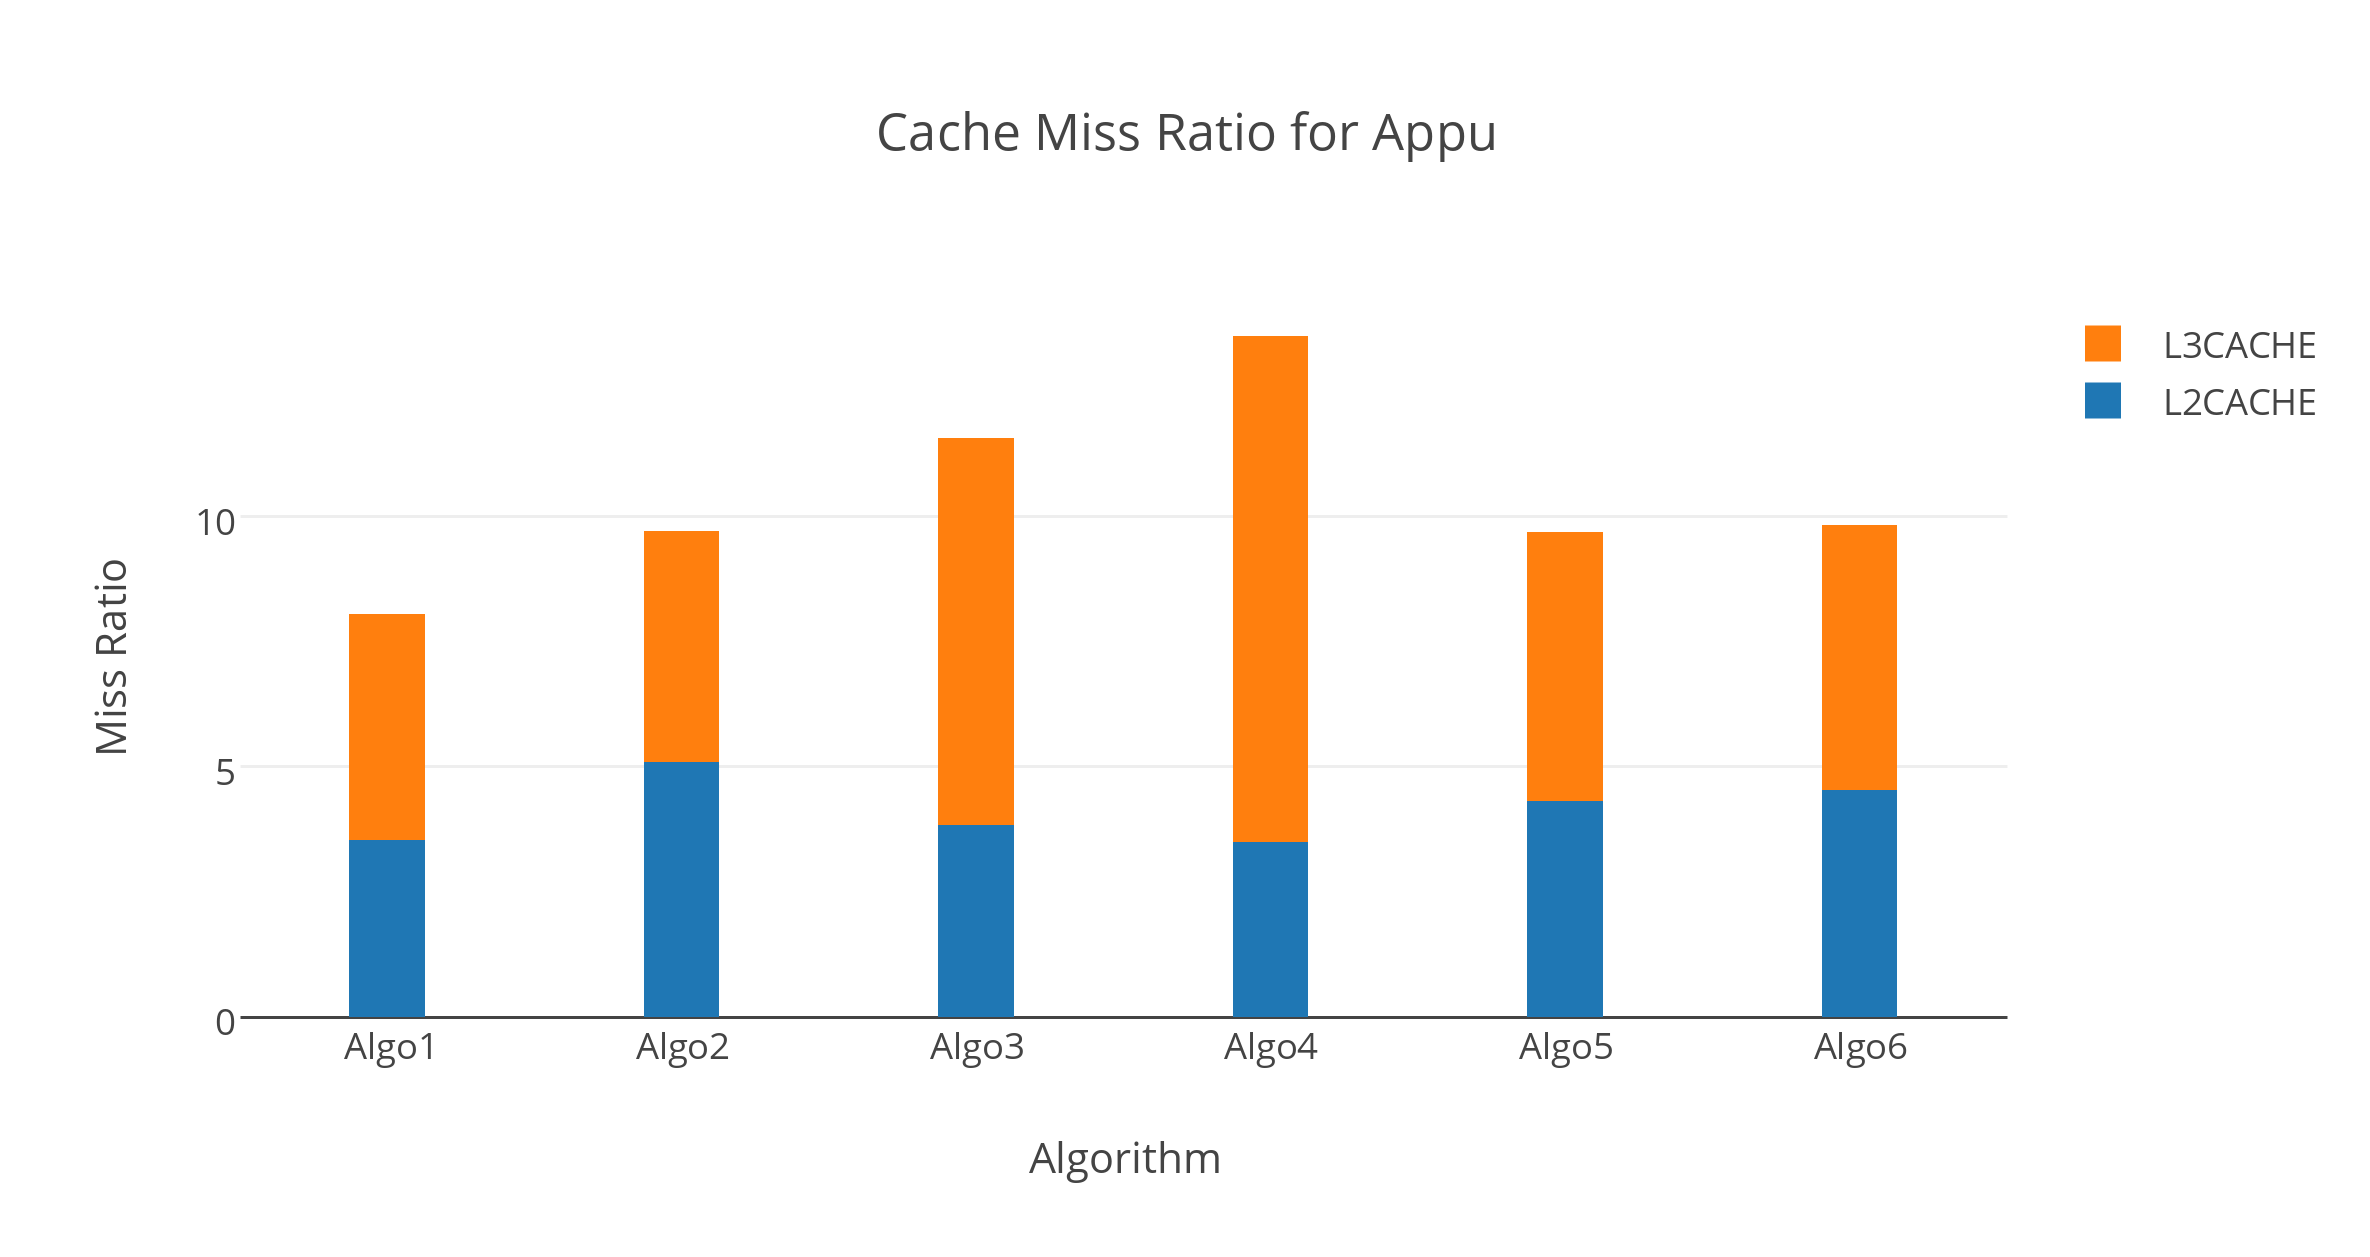
\includegraphics[width=0.5\textwidth]{figures/CacheMissRatioforAppu.eps}
    \caption{Cache-miss ratio for Appu}
    \label{fig:Appu-Cache Miss}
\end{figure}

\begin{figure}[t]
    \centering
    \includegraphics[width=0.5\textwidth]{figures/CacheMissRatioforDelaunay.eps}
    \caption{Cache-miss ratio for Delaunay}
    \label{fig:Delaunay-Cache Miss}
\end{figure}

\begin{figure}[t]
    \centering
    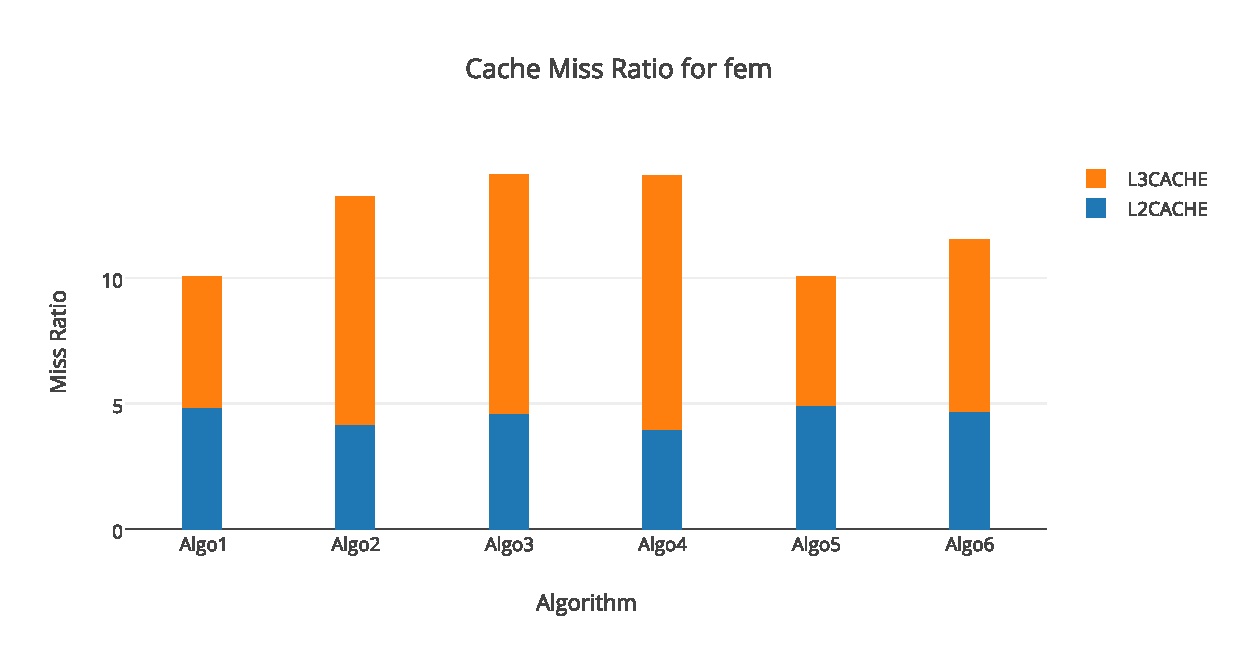
\includegraphics[width=0.5\textwidth]{figures/CacheMissRatioforFem.eps}
    \caption{Cache-miss ratio for Fem}
    \label{fig:Fem-Cache Miss}
\end{figure}

\begin{figure}[t]
    \centering
    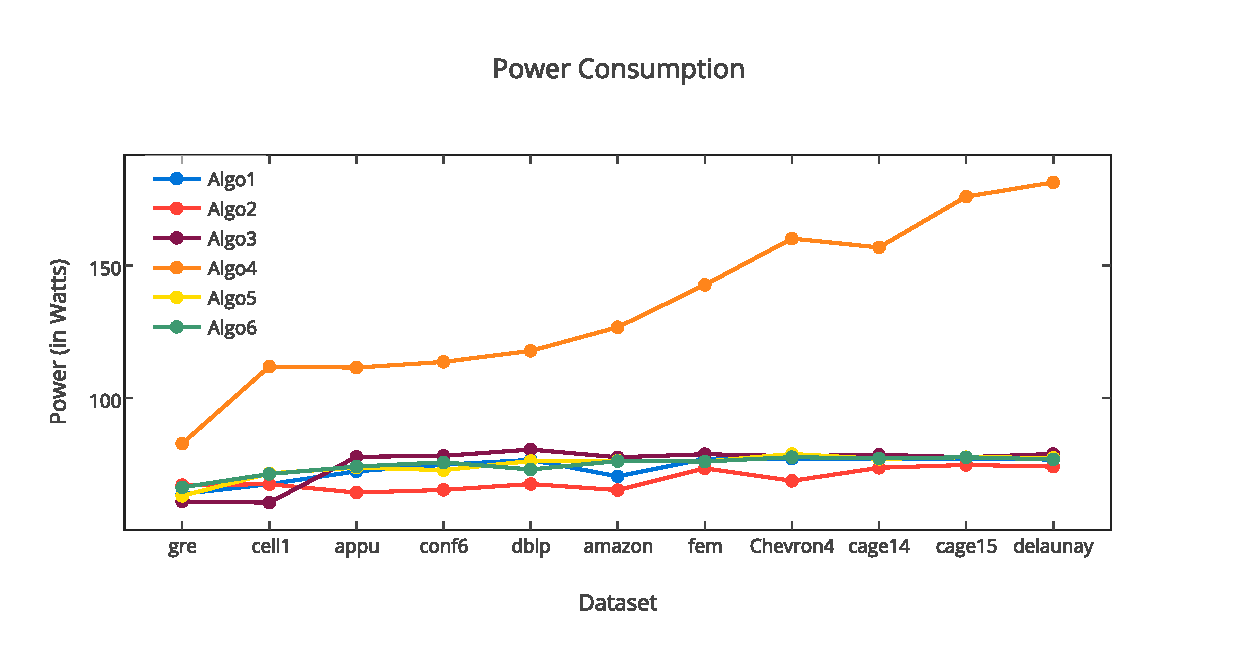
\includegraphics[width=0.5\textwidth]{figures/PowerConsumption.eps}
    \caption{Power Consumption}
    \label{fig:Power Consumption}
\end{figure}


\begin{figure}[t]
    \centering
    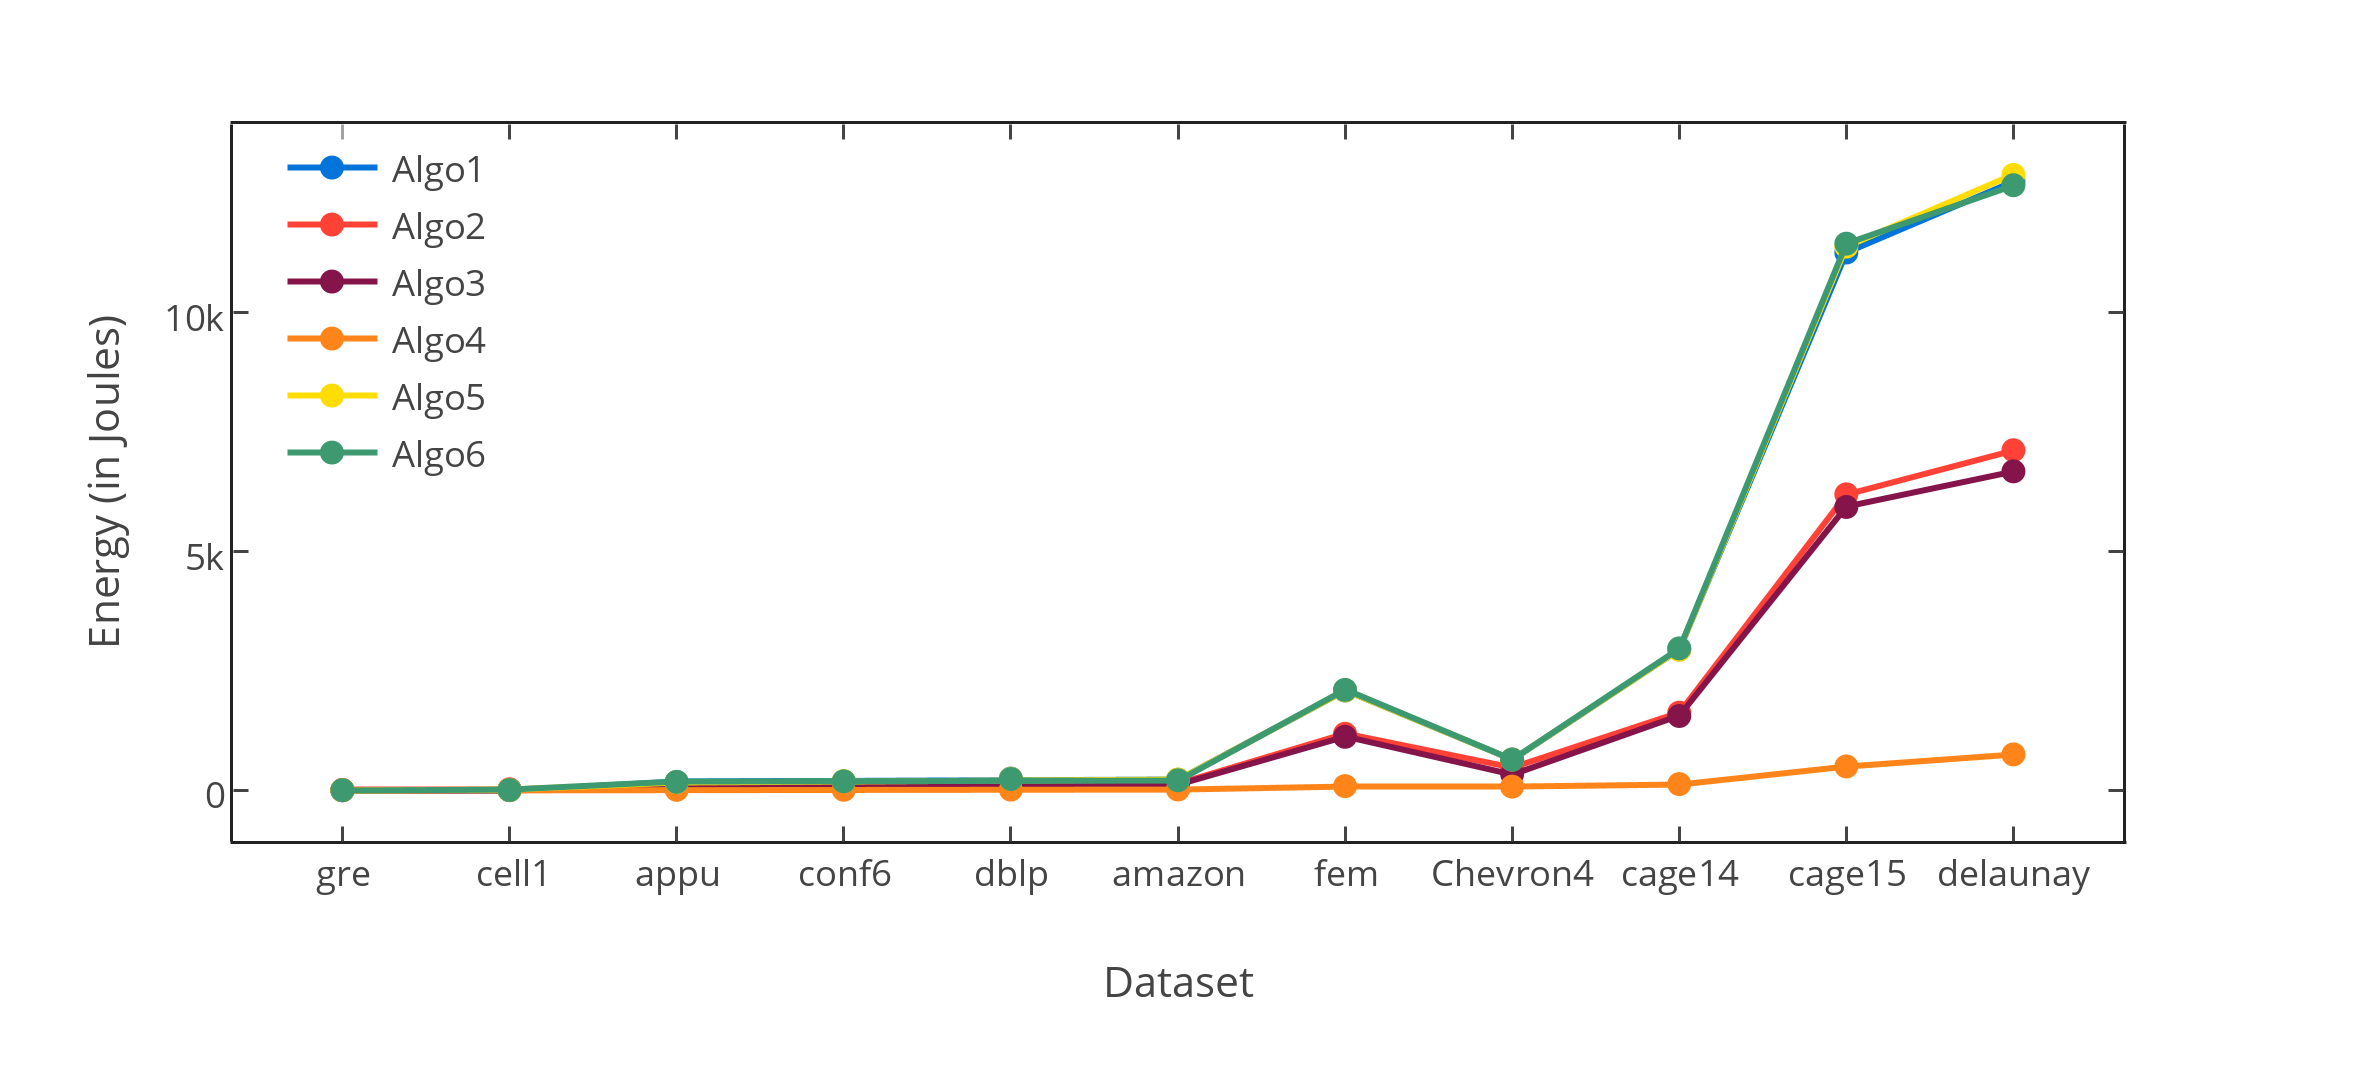
\includegraphics[width=0.5\textwidth]{figures/EnergyConsumption.eps}
    \caption{Energy Consumption}
    \label{fig:Energy Consumption}
\end{figure}


\begin{figure}[t]
    \centering
    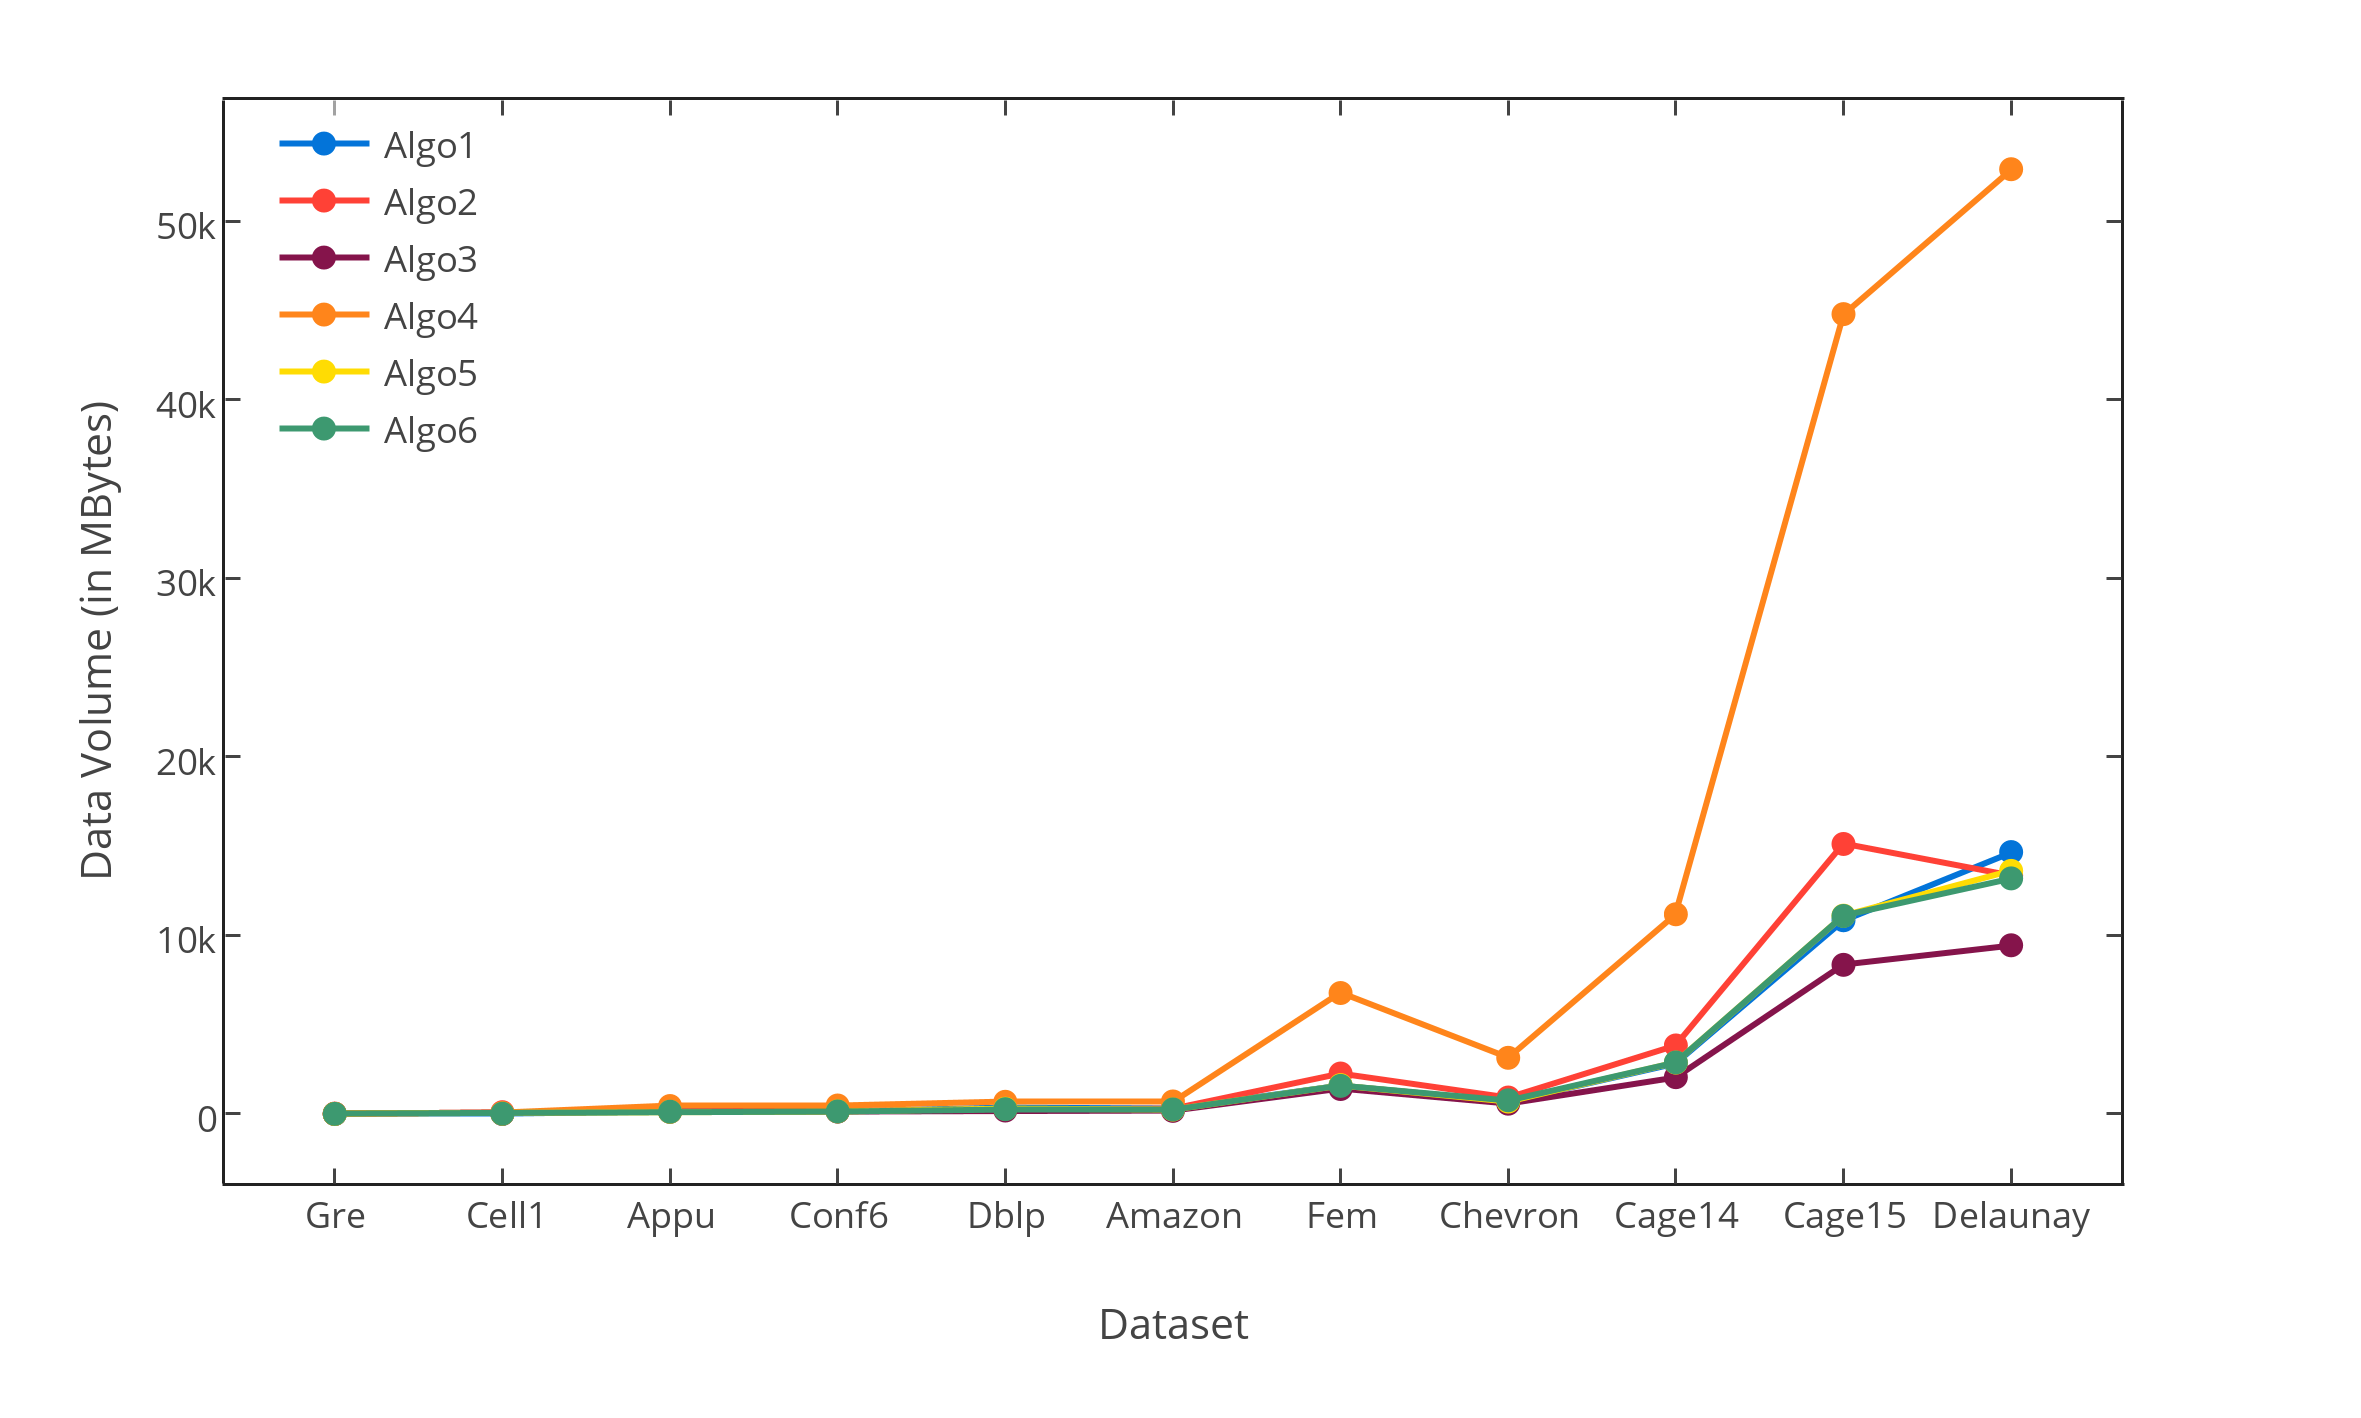
\includegraphics[width=0.5\textwidth]{figures/MEM-DataVolumeReadings.eps}
    \caption{MEM Consumption}
    \label{fig:MEM Consumption}
\end{figure}

\paragraph{MEM performance}
From Table~\ref{tab:Table3} we can see that Algo3 performs the best
for most of the times.

\paragraph{L2CACHE performance}
From Table~\ref{tab:Table6} we can see that Algo4 performs best for
most of the times.

\paragraph{L3CACHE performance}
From Table~\ref{tab:Table6} we can see that Algo1 performs best for
most of the times.

\paragraph{Energy efficiency}
From Table~\ref{tab:Table5} we can see that Algo4 performs best for
most of the times. It reduces the work by avoiding an the re-visit of
already explored nodes, so overall energy consumption is minimal.

\paragraph{POWER efficiency}
Normally a machine consumes a constant amount of power if operated
with default parameters. But from Table~\ref{tab:Table5} we can see
that \emph{Algo4} takes the highest amount of power. This behavior can
be attributed to its inherent design to exploit max amount of
parallelism from the hardware.  To verify this we used the same
CPU and thread parameters for each algorithm, still Algo4 consumes max
power.

























%%%%%%%%%%%%%%%%%%%%%%%%%%%%%%%%%%%%%%%%%%%%%%%%%%%%%%%%%%%%%%%%%%%%%%%%%%%%%%%
% Table(s) for results of current experiments
%%%%%%%%%%%%%%%%%%%%%%%%%%%%%%%%%%%%%%%%%%%%%%%%%%%%%%%%%%%%%%%%%%%%%%%%%%%%%%

\begin{table*}[th]
\small
\centering
%\begin{tabularx}{\linewidth}{|c|c|c|c|c|c|c|X|}

\begin{tabular}{ c|c|c|c|c|c|c|c|c| }
  \cline{2-9}
  & 
  \multicolumn{2}{c}{\textbf{$u_{1}$}} &
  \multicolumn{2}{|c}{\textbf{$u_{2}$}} &
  \multicolumn{2}{|c}{\textbf{$u_{3}$}} &
  \multicolumn{2}{|c|}{\textbf{root}}  \\
  \cline{2-9}
  \multicolumn{1}{c|}{} &
  with & without & with & without & with & without & with & without\\
  \multicolumn{1}{c|}{} &
  change & changes & changes & changes & changes & changes & changes &
  changes\\
  \hline
  \multicolumn{1}{|c|}{\textbf{create file}}
  & Y & Y & N & Y & N & Y & N & Y \\
  \hline
  \multicolumn{1}{|c|}{\textbf{create dir}}
  & Y & Y & N & Y & N & Y & N & Y \\
  \hline
  \multicolumn{1}{|c|}{\textbf{remove file}}
  & Y & Y & N & Y & N & Y & N & Y \\
  \hline
  \multicolumn{1}{|c|}{\textbf{remove dir}}
  & Y & Y & N & Y & N & Y & N & Y \\
  \hline
  \multicolumn{1}{|c|}{\textbf{create symlink}}
  & Y & Y & N & Y & N & Y & N & Y \\
  \hline
  \multicolumn{1}{|c|}{\textbf{read symlink}}
  & Y & Y & N & Y & N & Y & N & Y \\
  \hline
  \multicolumn{1}{|c|}{\textbf{write symlink}}
  & Y & Y & N & Y & N & Y & N & Y \\
  \hline
  \multicolumn{1}{|c|}{\textbf{create hardlink}}
  & Y & Y & N & Y & N & Y & N & Y \\
  \hline
  \multicolumn{1}{|c|}{\textbf{write hardlink}}
  & Y & Y & N & Y & N & Y & N & Y \\
  \hline
  \multicolumn{1}{|c|}{\textbf{stat}}
  & Y & Y & N & Y & N & Y & N & Y \\
  \hline
  \multicolumn{1}{|c|}{\textbf{change dir}}
  & Y & Y & N & Y & N & Y & N & Y \\
  \hline
  \multicolumn{1}{|c|}{\textbf{read file}}
  & Y & Y & N & Y & N & Y & N & Y \\
  \hline
  \multicolumn{1}{|c|}{\textbf{write file}}
  & Y & Y & N & Y & N & Y & N & Y \\
  \hline
  \multicolumn{1}{|c|}{\textbf{create tar}}
  & Y & Y & N & Y & N & Y & N & Y \\
  \hline
  \multicolumn{1}{|c|}{\textbf{untar}}
  & Y & Y & N & Y & N & Y & N & Y \\
  \hline
  \multicolumn{1}{|c|}{\textbf{make}}
  & Y & Y & N & Y & N & Y & N & Y \\
  \hline
  \multicolumn{1}{|c|}{\textbf{rename}}
  & Y & Y & N & Y & N & Y & N & Y \\
  \hline
\end{tabular}

%\end{tabularx}
\caption{\capfont Results of different file system operations for
different users, with and without the changes.}
\label{tab:results}
\end{table*}

%%%%%%%%%%%%%%%%%%%%%%%%%%%%%%%%%%%%%%%%%%%%%%%%%%%%%%%%%%%%%%%%%%%%%%%%%%%%%%
%% For Emacs:
% Local variables:
% fill-column: 70
% End:
%%%%%%%%%%%%%%%%%%%%%%%%%%%%%%%%%%%%%%%%%%%%%%%%%%%%%%%%%%%%%%%%%%%%%%%%%%%%%%
%% For Vim:
% vim:textwidth=70
%%%%%%%%%%%%%%%%%%%%%%%%%%%%%%%%%%%%%%%%%%%%%%%%%%%%%%%%%%%%%%%%%%%%%%%%%%%%%%
% LocalWords:  PEAFS PEAIO Lustre SBU HMC config

%%%%%%%%%%%%%%%%%%%%%%%%%%%%%%%%%%%%%%%%%%%%%%%%%%%%%%%%%%%%%%%%%%%%%%%%%%%%%%%
% Table(s) for results of current experiments
%%%%%%%%%%%%%%%%%%%%%%%%%%%%%%%%%%%%%%%%%%%%%%%%%%%%%%%%%%%%%%%%%%%%%%%%%%%%%%

\begin{table*}[th]
\small
\centering
%\begin{tabularx}{\linewidth}{|c|c|c|c|c|c|c|X|}

\begin{tabular}{ c|c|c|c|c|c|c| }
  \cline{2-7}
  & 
  \multicolumn{2}{c}{\textbf{root}} &
  \multicolumn{2}{|c}{\textbf{user1}} &
  \multicolumn{2}{|c|}{\textbf{root\_notallowed}}\\ 
  \cline{2-7}
  \multicolumn{1}{c|}{} &
  with & without & with & without & with & without\\
  \multicolumn{1}{c|}{} &
  changes & changes & changes & changes & changes & changes\\
  \hline
  \multicolumn{1}{|c|}{\textbf{xfstests}}
  & 56(68) & 56(68) & 32(68) & 32(68) & 0(68) & - \\
  \hline
  \multicolumn{1}{|c|}{\textbf{eCryptfs-tests}}
  & 25(25) & 25(25) & 22(25) & 22(25) & 0(25) & - \\
  \hline
\end{tabular}

%\end{tabularx}
\caption{\capfont Number of passed tests and total tests for
\emph{XFSTEST} and \emph{eCryptfs-tests} for different users, with and
without the changes.}
\label{tab:results-xfs}
\end{table*}

%%%%%%%%%%%%%%%%%%%%%%%%%%%%%%%%%%%%%%%%%%%%%%%%%%%%%%%%%%%%%%%%%%%%%%%%%%%%%%
%% For Emacs:
% Local variables:
% fill-column: 70
% End:
%%%%%%%%%%%%%%%%%%%%%%%%%%%%%%%%%%%%%%%%%%%%%%%%%%%%%%%%%%%%%%%%%%%%%%%%%%%%%%
%% For Vim:
% vim:textwidth=70
%%%%%%%%%%%%%%%%%%%%%%%%%%%%%%%%%%%%%%%%%%%%%%%%%%%%%%%%%%%%%%%%%%%%%%%%%%%%%%
% LocalWords:  PEAFS PEAIO Lustre SBU HMC config

%
%\paragraph{Evaluation Goals}
%We aimed to provide a correct working solution for eCryptfs with minimal
%performance overheads.
%
%\begin{itemize}
%\item
%\textbf{Correctness}\\
%Only the users that are allowed to access, should be able to access
%the file contents.  Other users should get a permission denied error
%irrespective of their privilege level.
%
%The user who is assigned the administrative role should be able to add
%or revoke permissions to other users in the system.
%
%Users without administrative privilege should not be able to change
%file access policy or gain illegal access.
%\item
%\textbf{Performance}\\ Performance of underlying file system should
%not suffer a penalty due to this extra security enforcement in
%eCryptfs.
%
%We keep the policy management separate from data path, so there is no
%overhead from management tasks on system performance.
%\item
%\textbf{Regression testing}\\ This change should not break any
%existing functionality in eCryptfs as well as the underlying file
%system.
%
%We have tested our changes with basic file operations like create
%file, directory, symlink, delete, rename, untar, kernel compilation.
%We also have run more comprehensive tests such as
%\emph{XFSTESTS}~\cite{xfstests} and eCryptfs-utils test scripts.
%\end{itemize}
%
%\paragraph{Evaluation Plan}
%We have run a set of testing tools along with our manually written
%tests.  The tools are \emph{XFSTESTS} and test scripts provided in
%eCriptfs-utils.  We have run these tools on both modified and
%unmodified eCryptfs kernel for different users with different
%privilege level.  We have tried to run the maximum number of tests
%from these tools, in case of a test failure we rerun it in isolation and
%identify the root cause of failure.  Test cases from these tools are
%sufficient, as they test for the functionality and regression of the file
%system.
%
%\paragraph{Experimental Setup}
%We have used a virtual machine with two Intel\textregistered
%Xeon\texttrademark dual-core 2.40GHz CPUs, and 8GB RAM.  The machine
%ran \mbox{Ubuntu} 14.04.1 with a vanilla 3.19.5 Linux Kernel.  We
%chose \mbox{Ubuntu} because it is freely available and the package
%eCryptfs-utils is installed by default.  For our experiments, we have
%4 users $u_1$, $u_2$, $u_3$ and a root user.  Only user $u_1$ is
%authorized to access encrypted files.  User $u_2$ is placed in sudoer
%list, $u_3$ is a normal user.  All users have intention to access the
%encrypted data, so we have 3 type of attackers and one authorized
%user.
%
%
%\begin{figure}[t]
%    \centering
%    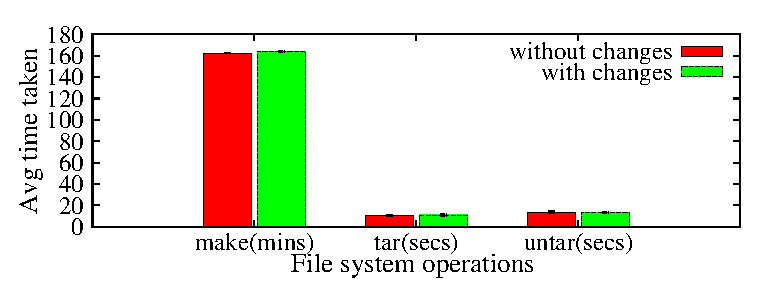
\includegraphics[width=0.5\textwidth]{figures/perf-results.eps}
%    \caption{eCryptfs performance comparison with and without our
%    changes for make, tar, untar operations.}
%    \label{fig:perf-results}
%\end{figure}
%
%
%\paragraph{Results}
%We ran basic file system operation for all four users mentioned above
%on the setup described.  We made changes to Linux Kernel 3.19.5.
%Table~\ref{tab:results} describes the results for all the file systems
%operations we ran.  Column 1 describes the file system operation.
%Column 2,3,4 shows results for users $u_1$, $u_2$, $u_3$ and root user
%respectively with and without our changes in Linux kernel.  \textbf{Y}
%indicates that the  operation ran successfully.  \textbf{N} indicates
%that the user was denied to run the corresponding commands inside the
%eCryptfs mount point.  We also ran some performance tests, such as
%make a Linux Kernel, tar/untar the source tree of Linux Kernel.
%Figure~\ref{fig:perf-results} shows that there is no significant
%performance overhead due to our changes.  The overhead for make workload
%is \emph{1.17\%} and for tar/untar is \emph{1.66\%}.
%
%We ran \emph{XFSTESTS} test-suite on Linux-3.19.5 vanilla kernel for
%\emph{eCryptfs} file system.  We used \emph{FSL} git repository of
%\emph{XFSTESTS} for our tests.  We modified the test-suite to support
%\emph{eCryptfs} file system.  These tests can be categorized in two
%categories, 1, without changes and 2, with changes in eCryptfs kernel
%code.  For category 1 we ran the test-suite for root user and a
%non-root user.  For category 2 we ran the test-suite for an allowed
%non-root user, and root user.  Then we added the root user to allowed
%users list and ran the test-suite again.  We compared the test results
%for both categories for each corresponding user.  We find there is no
%difference in the results.  We see that for category 2, when root user
%was not allowed to access eCryptfs file system, all tests failed.
%
%We also found new interesting bugs with eCryptfs file system.
%\begin{itemize}
%\item 
%\textbf{noatime mount option:} If the eCryptfs file system is mounted
%with noatime mount option, the access times for any file should never
%change.  But we see that there is no difference between if file system
%is mounted with noatime option or not.  The access time for files
%changes in both the cases.
%
%\item
%\textbf{Direct IO:} eCryptfs does not support direct IO.  So all the
%tests for direct IO failed.
%\item
%\textbf{File access timestamp Epoch:} Create a file in eCryptfs
%directory with creation time before epoch.  Check the time of last
%access as seconds since Epoch, it should be a negative value.  Now
%flush the cache by remounting the file system.  Now if we check again
%for the time of last access as seconds since Epoch, it should still be
%negative, but that is not the case here.
%\end{itemize}
%
%All the \emph{XFSTESTS} that failed can be assigned to the issues
%mentioned above.
%
%We also ran the default eCryptfs-test script found in eCryptfs utils.
%These tests include various file systems tests, such as file read,
%write, concurrent access, inode races, symlinks, file truncate.  These
%tests also include tests for already identified bugs in eCryptfs.
%These tests ensures that we did not break anything that was working
%before our changes.  For both the categories, we did not find any
%difference in the results for all the tests.  As expected for any
%non-allowed user all the tests in the script failed.
%
%Table~\ref{tab:results-xfs} shows the number of tests that passed from
%total number of tests for both the test-suites for various users.  We
%examined the failed tests and identified why some of \emph{XFSTESTS}
%failed.  The numbers show that there was nothing broken due to our
%changes.  Since many tests requires root permissions as these are
%kernel level tests, the amount of tests that failed for non-root user
%were considerably higher than that of root user.
%
%IOCTL interface is restricted to admin user.  For our experiments we
%hard coded a UID \mbox{1234} as admin user in eCryptfs kernel.  We
%created a user with UID \mbox{1234} using adduser(1) utility.  At
%mount time only admin user is added to the list of allowed users.
%Root can mount the file system but cannot access the files within the
%mount point, as it is not part of allowed list.  At this point only
%admin user can perform file operation and user management activity.
%Once the admin added a user to the set of allowed users, that user can
%perform file operation.  Still user management operations like
%list\_users/allow\_user/revoke\_user is restricted to admin user.
%
%We tested IOCTL interface via multiple users like admin, user1, user2,
%root.  We observed that only admin user was able to successfully run
%the IOCTL commands, other users including root got permission denied
%error.  Since admin role is non-revocable, even the admin user cannot
%revoke itself.  Admin user cannot add any users to the allowed list
%once the list was full, too many users error is returned.  We verified
%that the file operation path was being properly affected by the
%changes done via IOCTL interface.
%
%%%%%%%%%%%%%%%%%%%%%%%%%%%%%%%%%%%%%%%%%%%%%%%%%%%%%%%%%%%%%%%%%%%%%%%%%%%%%%
%% For Emacs:
% Local variables:
% fill-column: 70
% End:
%%%%%%%%%%%%%%%%%%%%%%%%%%%%%%%%%%%%%%%%%%%%%%%%%%%%%%%%%%%%%%%%%%%%%%%%%%%%%%
%% For Vim:
% vim:textwidth=70
%%%%%%%%%%%%%%%%%%%%%%%%%%%%%%%%%%%%%%%%%%%%%%%%%%%%%%%%%%%%%%%%%%%%%%%%%%%%%%
% LocalWords:
